\documentclass{beamer}
\usepackage[italian]{babel}
\usepackage{graphicx}
\usepackage{bm}
\usepackage{hyperref}
\usepackage[italian]{babel}
\RequirePackage{palatino}
\RequirePackage[utf8]{inputenc}
\RequirePackage[T1]{fontenc}

\usefonttheme{serif}
\graphicspath{ {./pic/} }

\newcommand{\makepart}[1]{ % For convenience
\part{#1} \frame{\partpage}
}
\usepackage{styles/elegantmacros}
\usepackage{styles/bussproofs}
\usefolder{styles}
\usetheme[style=blue]{elegant}

\title[
]{Isomorfismo di Curry-Howard}

\subtitle{Dove la Logica e l'Informatica si incontrano}

\author[
]{
    Mattia Girolimetto
}

\institute{
Relazione per il corso 85001 - Metodi logici per la Filosofia \\
    Alma Mater Studiorum, Università di Bologna}
\date{\today}

\begin{document}
\begin{frame}
  \titlepage
\end{frame}

\begin{frame}{Indice}
  \tableofcontents[part=1]
  \tableofcontents[part=2]
  \tableofcontents[part=3]
  \tableofcontents[part=4]
\end{frame}


\begin{frame}{}
\begin{center}
  Questa presentazione sarà presto disponibile all'url $http://www.github.com/specialfish9/curry-howard$
\end{center}
\end{frame}


\makepart{Logica proposizionale}
\section{Logica proposizionale}

\begin{frame}{Formule \& regole}
\begin{itemize}
  \item \textit{Variabili} $A, B, C, ...$
  \item \textit{Falso} $\bot$
  \item \textit{Implicazione} $\rightarrow$
\end{itemize}
  \begin{columns}
    \column{0.33\textwidth} 
  \begin{prooftree}
    \AxiomC{}
    \RightLabel{Axiom}
    \UnaryInfC{$\Gamma, F, \Gamma' \vdash F$}
  \end{prooftree}

    \column{0.33\textwidth} 
  \begin{prooftree}
    \AxiomC{$\Gamma, F \vdash G$}
    \RightLabel{$\rightarrow i$}
    \UnaryInfC{$\Gamma \vdash F \rightarrow G$}
  \end{prooftree}

    \column{0.33\textwidth} 
  \begin{prooftree}
    \AxiomC{$\Gamma \vdash F \rightarrow G$}
    \AxiomC{$\Gamma \vdash F$}
    \RightLabel{$\rightarrow e$}
    \BinaryInfC{$\Gamma \vdash G$}
  \end{prooftree}
  
\end{columns}

  % TODO add falso
\end{frame}

\makepart{Lambda calcolo}
\section{Lambda calcolo}

\begin{frame}{Cos'è il lambda calcolo?}
\begin{itemize}
  \item E' un sistema formale creato da Alonzo Church nel 1936
  \item Usato per dimostrare l'indecidibilità del \textit{Entscheidungsproblem}
    ("problema di decisone")
\end{itemize}
\begin{center}
  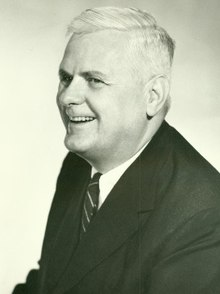
\includegraphics[scale=0.70]{8.jpg}
\end{center}
\end{frame}

\begin{frame}{L'importanza del lamda calcolo}
Il lambda calcolo trova applicazioni in diversi campi 
\begin{itemize}
  \item Svolge un ruolo chiave nella \textit{teoria della calcolabilità} 
  \item Ha dato origine al paradigma funzionale nella \textit{teoria dei linguaggi
        di programmazione}
  \item La sua versione tipata, grazie all'isomorfismo di Curry-Howard, assume
        una grande importanza nella \textit{teoria della dimostrazione}
\end{itemize}
\end{frame}

\begin{frame}{Lambda calcolo e Informatica}
\begin{center}
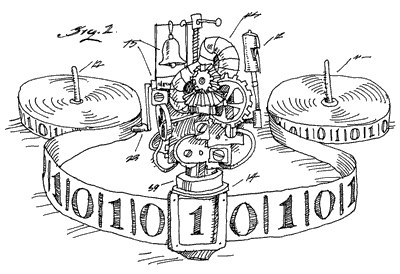
\includegraphics[scale=0.60]{3.png}
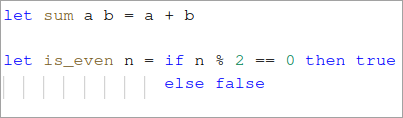
\includegraphics[scale=0.60]{4.png}
\end{center}
\end{frame}

\begin{frame}{Intuizione}
\begin{center}
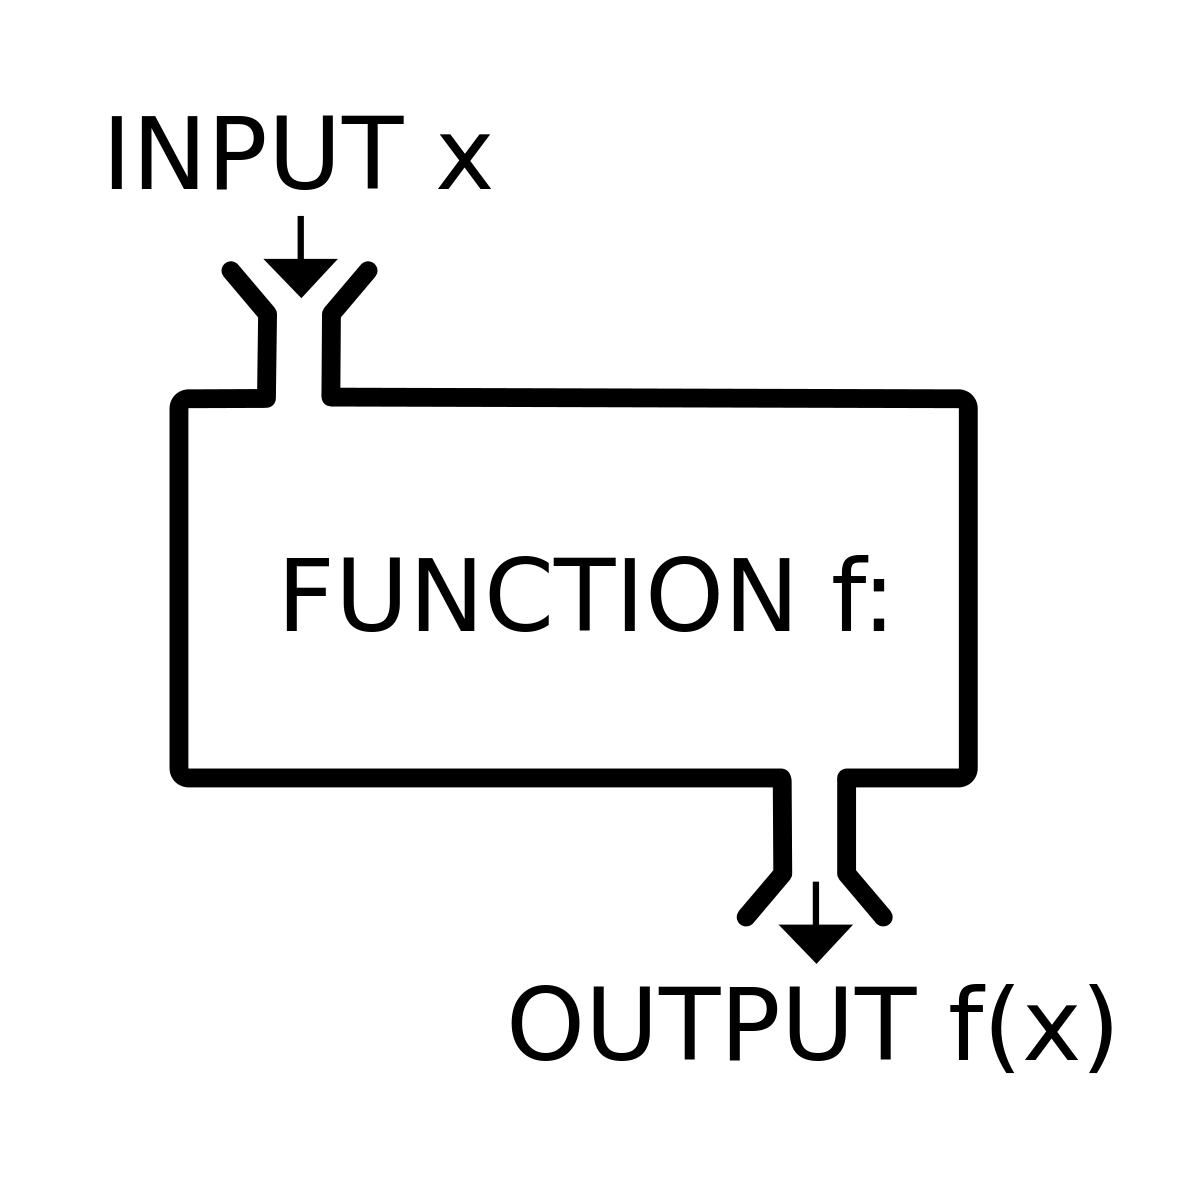
\includegraphics[scale=0.15]{9.png}
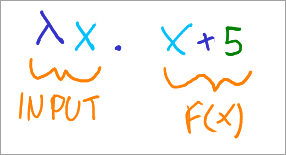
\includegraphics[scale=0.7]{10.png}
\end{center}
\end{frame}

\begin{frame}{Espressioni Lambda}
  Sono composte di:
\begin{itemize}
    \item \textit{Variabili} $x, y, ...$
    \item \textit{Simboli di astrazione} $\lambda$ (lambda) e $.$ (dot)
    \item \textit{Parentesi} $()$
\end{itemize}
\end{frame}
  
\begin{frame}{Espressioni Lambda}

  \begin{definition}[Espressioni Lambda (o Lambda-Termini)]
  L'insieme di tutte le espressioni lambda $\Lambda$ è definito induttivamente 
  come segue:
  \begin{itemize}
    \item Se $x$ è una variabile allora $x \in \Lambda$
    \item Se $x$ è una variabile e $M \in \Lambda$ allora $(\lambda x.M) \in
      \Lambda$ (\textit{Astrazione} o \textit{funzione})
    \item Se $M, N \in \Lambda$ allora $(M$ $N) \in \Lambda$ (\textit{Applicazione})
  \end{itemize}
\end{definition}

  \begin{exampleblock}{Esempi}

\begin{itemize}
  \item  $\lambda x . x$ 
  \item $(\lambda x. x)$ $y$
  \item  $\lambda x . (\lambda y. y)$ 
  \item  $\lambda x . (\lambda y. (\lambda z. z))$ 
\end{itemize}
\end{exampleblock}
\end{frame}

\begin{frame}{Disclaimer}
\begin{itemize}
  \item Nel Lambda Calcolo definito da Church \textbf{non esiste} il concetto
    di numero o di valore di verità, e non esistono peratori aritmetici o logici.
    Esistono solo le funzioni espresse come lambda termini.
  \item Tuttavia è comunque possibile rappresentare questi concetti tramite delle
    \textit{codifiche}, la più famosa è quella di Church stesso.
  \item Per semplicità oggi assumiamo che numeri, valori di verità e operatori
    aritmetici e logici siano già definiti.
  \item Se qualcuno è interessato a capire meglio come funzionano queste codifiche
    consiglio \alert{\href{https://www.youtube.com/watch?v=RsO_sfHtXCM&ab_channel=Truttle1}{
      questo }} simpatico video.
\end{itemize}

\end{frame}


\begin{frame}{Sostituizione}
\begin{definition}[Sostituzione]
  L'operazione di \textit{sostituzione} di una variabile $u$ con una variabile 
  $v$ in un lambda-termine è così definita:
\begin{itemize}
  \item $x[v/u] = v$ se $x = u$
  \item $x[v/u] = x$ se $x \ne u$
  \item $(\lambda x.M)[v/u]$ = $\lambda x[v/u].M[v/u]$
  \item $(M$ $N)[v/u]=M[v/u]$ $N[v/u]$ 
\end{itemize}

\end{definition}
\end{frame}

\begin{frame}{$\beta$-reduction}
  \begin{definition}[$\beta$-reduction]
    $(\lambda x . M) N \rightarrow_\beta M[N/x]$ 
  \end{definition}


    \begin{exampleblock}{Esempi}
      $(\lambda x. x + 2) 5 \rightarrow_\beta 5 + 2$ \\
      $(\lambda x . x ) (\lambda y . y + 1) \rightarrow_\beta \lambda y . y + 1$ 
    \end{exampleblock}


  \end{frame}

\begin{frame}{Il calcolo all'opera}

  \begin{minipage}[b]{2\textwidth}
  \begin{exampleblock}{Funzione Identità}
    $id := \lambda x .x $ \\
    $id$ 2 $= (\lambda x .x) 2 \longrightarrow_\beta 2$
  \end{exampleblock}

  \begin{exampleblock}{Funzione Quadrato}
    $square := \lambda x . x * x$ \\
    $square$ 2 $= (\lambda x. x * x) 2 \longrightarrow_\beta 2 * 2 = 4$ \\
  \end{exampleblock}

  \begin{exampleblock}{Funzione Somma}
    $sum := \lambda x .(\lambda y . x + y)$ \\
    $sum$ 2 4 $= ((\lambda x. (\lambda y . x + y))4)2  \longrightarrow_\beta (\lambda y . 2 + y ) 4 \longrightarrow_\beta 2 + 4 = 6$ \\
  \end{exampleblock}
  \end{minipage}
\end{frame}

\begin{frame}{Quanto vale?}
Sia $idk := \lambda x .(\lambda y. x $ $y)$. \alert{Quanto vale $idk$ $(\lambda z. z * 2)$  $5$?} \\
\begin{center}

\includegraphics[scale=0.40]{5.jpg}
\end{center}
\end{frame}

\begin{frame}{Quanto vale?}
Sia $idk := \lambda x .(\lambda y. x $ $y)$. \alert{Quanto vale $idk$ $(\lambda z. z * 2)$  $5$?} \\
\alert{\textbf{Soluzione:}} \\
  $idk$ $(\lambda z. z * 2)$ $5$  \\
  $= ((\lambda x . (\lambda y . x$ $y)) 5) (\lambda z. z * 2)$ \\
  $\longrightarrow_\beta (\lambda y . (\lambda z . z * 2) y) 5$ \\
  $\longrightarrow_\beta (\lambda z . z * 2) 5$ \\
  $\longrightarrow_\beta 5 * 2$ \\
  $= 10$
\end{frame}

\makepart{Lambda calcolo tipato semplice}
\section{Lambda calcolo tipato semplice}

\begin{frame}{Lambda-termini e tipi}
  \begin{definition}[Tipo]
    Sia $B$ l'insieme di tutti i \textit{tipi base} (ad esempio $\mathbb{N},
    \mathbb{R},  \mathbb{B}$...). Definiamo un \alert{\textbf{tipo}} come:
    \begin{itemize}
      \item $\tau \in B$
      \item $(\sigma \rightarrow \tau)$ con $\sigma, \tau$ tipi (\textit{tipo funzione})
    \end{itemize}
  \end{definition}
\end{frame}

\begin{frame}{Lambda-termini e tipi}
  \begin{definition}[Assegnazione di tipo]
    Un'assegnazione di tipo è un'espressione $(t : \tau)$ dove $t$ è un lambda-termine
    e $\tau$ è un tipo.
  \end{definition}
  \begin{exampleblock}{Esempio}
    \begin{columns}
      \column{0.20\textwidth} 
      $x : \mathbb{N}$
      \column{0.30\textwidth} 
      $(\lambda x: \mathbb{R}. falso): (\mathbb{R} \rightarrow \mathbb{B})$
      \column{0.30\textwidth} 
      $(f$ $y) : \mathbb{B}$
    \end{columns}
  \end{exampleblock}

  \begin{definition}[Contesto di tipo]
    Un contesto di tipo $\Gamma$ è un insieme finito di assegnazioni di tipi a
    variabili, tale che sia \textit{consistente}: ogni variabile ha associato un
    e un solo tipo.
  \end{definition}
  \begin{exampleblock}{Esempio}
    $\Gamma =\{x: \mathbb{N}, y: \mathbb{B}, z: \mathbb{R} \rightarrow \mathbb{B}\}$
  \end{exampleblock}
\end{frame}

\begin{frame}{Che tipo ha $(\lambda x: \mathbb{N}. (\lambda y: \mathbb{R}. true))$?}
\begin{center}

\includegraphics[scale=0.40]{5.jpg}
\end{center}
\end{frame}

\begin{frame}{Che tipo ha $(\lambda x: \mathbb{N}. (\lambda y: \mathbb{R}. true))$?}
\begin{center}
  $(\lambda x: \mathbb{N} (\lambda y: \mathbb{R}. true)) : \mathbb{N} \rightarrow (
  \mathbb{R} \rightarrow \mathbb{B})$
\end{center}
\end{frame}

\begin{frame}{Regole di tipaggio}
  \begin{prooftree}
    \AxiomC{}
    \RightLabel{Var}
    \UnaryInfC{$\Gamma, x: \tau, \Gamma' \vdash x: \tau$}
  \end{prooftree}
  \begin{prooftree}
    \AxiomC{$\Gamma, x : \sigma \vdash M: \tau$}
    \RightLabel{Fun}
    \UnaryInfC{$\Gamma \vdash (\lambda x:\sigma.M) : \sigma \rightarrow \tau$}
  \end{prooftree}
  \begin{prooftree}
    \AxiomC{$\Gamma \vdash f: \sigma \rightarrow \tau$}
    \AxiomC{$\Gamma \vdash x: \sigma$}
    \RightLabel{App}
    \BinaryInfC{$\Gamma \vdash (f$ $x) : \tau$}
  \end{prooftree}
\end{frame}

\makepart{L'isomorfismo di Curry-Howard}
\section{L'isomorfismo di Curry-Howard}
\begin{frame}{L'Isomorfismo di Curry-Howard}
\begin{itemize}
  \item Scoperto dal matematico Haskell Curry e dal logico William Alvin Howard.
  \item Suggerito per la prima volta da Curry e formalizzato in un momento successivo
    da Howard.
  \item Evidenzia una relazione diretta tra programmi e prove formali.
\end{itemize}

\begin{center}
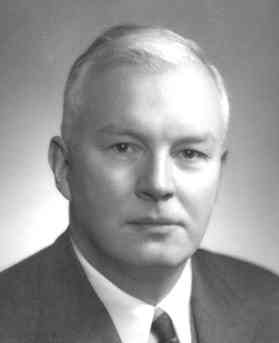
\includegraphics[scale=0.455]{1.jpg}
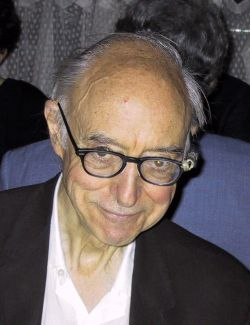
\includegraphics[scale=2]{2.jpg}
\end{center}
\end{frame}


\begin{frame}{Isomorfismo???}
    
  \begin{columns}
    \column{0.33\textwidth} 

  \begin{prooftree}
    \AxiomC{}
    \RightLabel{Axiom}
    \UnaryInfC{$\Gamma, F, \Gamma' \vdash F$}
  \end{prooftree}

  \begin{prooftree}
    \AxiomC{}
    \RightLabel{Var}
    \UnaryInfC{$\Gamma x : \tau \Gamma' \vdash x: \tau$}
  \end{prooftree}

    \column{0.33\textwidth} 
  \begin{prooftree}
    \AxiomC{$\Gamma, F \vdash G$}
    \RightLabel{$\rightarrow i$}
    \UnaryInfC{$\Gamma \vdash F \rightarrow G$}
  \end{prooftree}

  \begin{prooftree}
    \AxiomC{$\Gamma, x : \sigma \vdash M: \tau$}
    \RightLabel{Fun}
    \UnaryInfC{$\Gamma \vdash (\lambda x:\sigma.M) : \sigma \rightarrow \tau$}
  \end{prooftree}

  \column{0.33\textwidth} 
  \begin{prooftree}
    \AxiomC{$\Gamma \vdash F \rightarrow G$}
    \AxiomC{$\Gamma \vdash F$}
    \RightLabel{$\rightarrow e$}
    \BinaryInfC{$\Gamma \vdash G$}
  \end{prooftree}

  \begin{prooftree}
    \AxiomC{$\Gamma \vdash f: \sigma \rightarrow \tau$}
    \AxiomC{$\Gamma \vdash x: \sigma$}
    \RightLabel{App}
    \BinaryInfC{$\Gamma \vdash (f$ $x) : \tau$}
  \end{prooftree}

  \end{columns}
\end{frame}

\begin{frame}{Isomorfismo???}
    
  \begin{columns}
    \column{0.33\textwidth} 

  \begin{prooftree}
    \AxiomC{}
    \RightLabel{Axiom}
    \UnaryInfC{$\Gamma, F, \Gamma' \vdash F$}
  \end{prooftree}

  \begin{prooftree}
    \AxiomC{}
    \RightLabel{Var}
    \UnaryInfC{$\Gamma, x:F, \Gamma' \vdash x: F$}
  \end{prooftree}

    \column{0.33\textwidth} 
  \begin{prooftree}
    \AxiomC{$\Gamma, F \vdash G$}
    \RightLabel{$\rightarrow i$}
    \UnaryInfC{$\Gamma \vdash F \rightarrow G$}
  \end{prooftree}

  \begin{prooftree}
    \AxiomC{$\Gamma, x : F \vdash M: G$}
    \RightLabel{Fun}
    \UnaryInfC{$\Gamma \vdash (\lambda x:F .M) : F \rightarrow G$}
  \end{prooftree}

  \column{0.33\textwidth} 
  \begin{prooftree}
    \AxiomC{$\Gamma \vdash F \rightarrow G$}
    \AxiomC{$\Gamma \vdash F$}
    \RightLabel{$\rightarrow e$}
    \BinaryInfC{$\Gamma \vdash G$}
  \end{prooftree}

  \begin{prooftree}
    \AxiomC{$\Gamma \vdash f: F \rightarrow G$}
    \AxiomC{$\Gamma \vdash x: F$}
    \RightLabel{App}
    \BinaryInfC{$\Gamma \vdash (f$ $x) : G$}
  \end{prooftree}

  \end{columns}
\end{frame}

\begin{frame}{Isomorfismo!!!}
    
  \begin{columns}
    \column{0.33\textwidth} 

  \begin{prooftree}
    \AxiomC{}
    \RightLabel{Axiom}
    \UnaryInfC{$\Gamma, F, \Gamma' \vdash F$}
  \end{prooftree}

  \begin{prooftree}
    \AxiomC{}
    \RightLabel{Var}
    \UnaryInfC{$\alert{\boldsymbol{\Gamma,}} x: \alert{\boldsymbol{F, \Gamma' \vdash}} x: \alert{\textbf{F}}$}
  \end{prooftree}

    \column{0.33\textwidth} 
  \begin{prooftree}
    \AxiomC{$\Gamma, F \vdash G$}
    \RightLabel{$\rightarrow i$}
    \UnaryInfC{$\Gamma \vdash F \rightarrow G$}
  \end{prooftree}

  \begin{prooftree}
    \AxiomC{$\alert{\boldsymbol{\Gamma}}, x : \alert{\textbf{F}} \alert{\boldsymbol{\vdash}} M: \alert{\textbf{G}}$}
    \RightLabel{Fun}
    \UnaryInfC{$\alert{\boldsymbol{\Gamma}} \alert{\boldsymbol{\vdash}} (\lambda x:F .M) : \alert{\textbf{F}} \alert{\boldsymbol{\rightarrow}} \alert{\textbf{G}}$}
  \end{prooftree}

  \column{0.33\textwidth} 
  \begin{prooftree}
    \AxiomC{$\Gamma \vdash F \rightarrow G$}
    \AxiomC{$\Gamma \vdash F$}
    \RightLabel{$\rightarrow e$}
    \BinaryInfC{$\Gamma \vdash G$}
  \end{prooftree}

  \begin{prooftree}
    \AxiomC{$\alert{\boldsymbol{\Gamma \vdash}} f: \alert{\textbf{F}} \alert{\boldsymbol{\rightarrow}} \alert{\textbf{G}}$}
    \AxiomC{$\alert{\boldsymbol{\Gamma \vdash}} x: \alert{\textbf{F}}$}
    \RightLabel{App}
    \BinaryInfC{$\alert{\boldsymbol{\Gamma \vdash}} (f$ $x) : \alert{\textbf{G}}$}
  \end{prooftree}

  \end{columns}
\end{frame}

\begin{frame}{Isomorfismo!!!}
\begin{center}
  \begin{tabular}{ | c | c |}
    \hline
    \alert{\textbf{LOGICA}} & \alert{\textbf{INFORMATICA}} \\
    \hline
    Formule & Tipi\\
    \hline
    Prove & Programmi \\
    \hline
    Verifica di una prova & Verifica di tipo\\
    \hline
  \end{tabular}
\end{center}
\end{frame}

\begin{frame}{Isomorfismo!!!}
\begin{center}
  \begin{tabular}{ | c | c |}
    \hline
    \alert{\textbf{LOGICA}} & \alert{\textbf{INFORMATICA}} \\
    \hline
    $\top$ & Tipo unit \\
    \hline
    $\bot $ & Tipo vuoto/void \\
    \hline
   $\wedge$ & Tipi prodotto \\  
    \hline
   $\vee$ & Tipi somma \\
    \hline
   $\Rightarrow$ & Funzioni \\ 
    \hline
   $\exists$ & Tipi $\Sigma$ \\ 
    \hline
    $\forall $ & Tipi dipendenti (tipi $\Pi$)\\ 
    \hline

  \end{tabular}
\end{center}
\end{frame}


\begin{frame}{Isomorfismo e Logica Modale}
\begin{center}
   $\Box \longleftrightarrow $ staged computation \\
   $\Diamond \longleftrightarrow $ tipi monadici
\end{center}

\begin{itemize}
  \item \href{https://www.cs.cmu.edu/~fp/papers/mscs00.pdf}{Davies, Rowan;
    Pfenning, Frank(2001), "A Judgmental Reconstruction of Modal Logic"}
  \item  \href{https://www.cs.cmu.edu/~fp/papers/jacm00.pdf}{Davies, Rowan; Pfenning, Frank (2001), "A Modal Analysis of Staged Computation"}
\end{itemize}
\end{frame}


\begin{frame}{L'isomorfismo nella pratica}
\begin{itemize}
  \item L'isomorfismo ha permesso lo sviluppo di diversi verificatori di prove.
  \item Ne è esempio il software \alert{\href{https://github.com/sacerdot/matita}{matita}}, sviluppato a Bologna! 
\end{itemize}
\begin{center}

\includegraphics[scale=0.50]{7.png}
\end{center}
\end{frame}



\begin{frame}{Non c'è due senza tre}
\begin{itemize}
  \item  Negli anni settanta Joachim Lambek estende l'isomorfismo alla \textit{
      teoria delle categorie}.
\begin{center}

\includegraphics[scale=0.45]{11.jpg}
\end{center}
  \item Ma questa è un altra storia....
\end{itemize}

\end{frame}


\begin{frame}{Domande?}
\begin{center}

\includegraphics[scale=0.20]{12.png}
\end{center}
\end{frame}


\begin{frame}{Bibliografia/sitografia}

\begin{itemize}
  \item http://www.di.unito.it/~curzi/isomorfismo\%20di\%20Curry-Howard-Lambek.pdf 
  \item \href{https://www.cs.cmu.edu/~fp/papers/mscs00.pdf}{Davies, Rowan;
    Pfenning, Frank(2001), "A Judgmental Reconstruction of Modal Logic"}
  \item  \href{https://www.cs.cmu.edu/~fp/papers/jacm00.pdf}{Davies, Rowan; Pfenning, Frank (2001), "A Modal Analysis of Staged Computation"}
\end{itemize}
\end{frame}




\end{document}
